% !TeX root = ../../navier-stokes-manuscript.tex
\begin{figure}[!htbp]
  \centering
  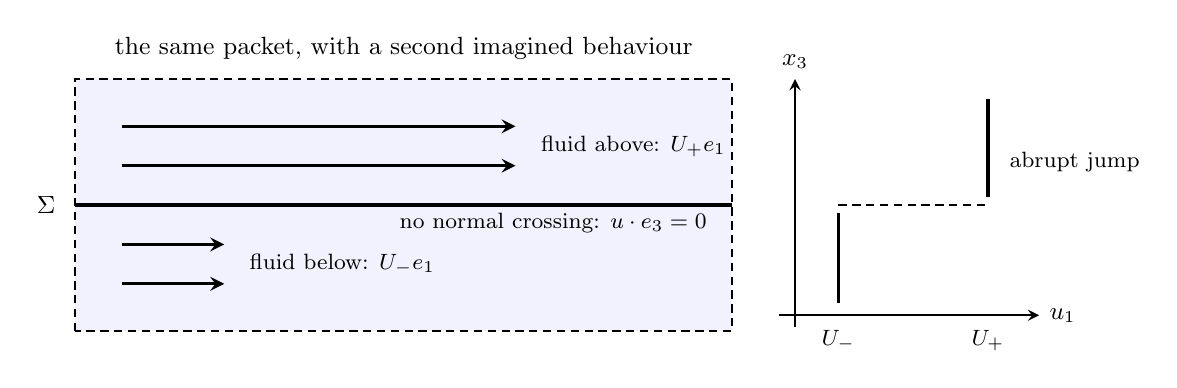
\begin{tikzpicture}[
    x=1cm,
    y=1cm,
    >=stealth,
    velocity/.style={->,very thick},
    smalllabel/.style={font=\small},
    tinylabel/.style={font=\footnotesize}
  ]
    \fill[blue!5]
      (0.50,0.65) rectangle (8.85,3.85);
    \draw[densely dashed,thick]
      (0.50,0.65) rectangle (8.85,3.85);
    \draw[very thick] (0.50,2.25) -- (8.85,2.25);
    \node[smalllabel,anchor=east] at (0.38,2.25) {\(\Sigma\)};

    \draw[velocity] (1.10,1.25) -- (2.40,1.25);
    \draw[velocity] (1.10,1.75) -- (2.40,1.75);
    \draw[velocity] (1.10,2.75) -- (6.10,2.75);
    \draw[velocity] (1.10,3.25) -- (6.10,3.25);

    \node[tinylabel,anchor=west] at (6.30,3.00)
      {fluid above: \(U_+e_1\)};
    \node[tinylabel,anchor=west] at (2.60,1.50)
      {fluid below: \(U_-e_1\)};
    \node[smalllabel,anchor=south] at (4.68,3.98)
      {the same packet, with a second imagined behaviour};
    \node[tinylabel,anchor=east] at (8.65,2.02)
      {no normal crossing: \(u\cdot e_3=0\)};

    \draw[->,thick] (9.65,0.70) -- (9.65,3.85)
      node[above,smalllabel] {\(x_3\)};
    \draw[->,thick] (9.45,0.85) -- (12.75,0.85)
      node[right,smalllabel] {\(u_1\)};
    \draw[very thick] (10.20,1.00) -- (10.20,2.15);
    \draw[very thick] (12.10,2.35) -- (12.10,3.60);
    \draw[densely dashed] (10.20,2.25) -- (12.10,2.25);
    \node[tinylabel,anchor=north] at (10.20,0.78) {\(U_-\)};
    \node[tinylabel,anchor=north] at (12.10,0.78) {\(U_+\)};
    \node[tinylabel,anchor=west] at (12.25,2.80)
      {abrupt jump};
  \end{tikzpicture}
  \caption{Board-like motion imagined inside the same fluid packet.
  The dashed outline is not a wall, and the two regions are not separate bodies.
  The one velocity field jumps tangentially across \(\Sigma\), so this profile is nonsmooth even though its normal flow remains zero.}
  \label{fig:BoardLikeSlip}
\end{figure}
